    Let $h = \ceil{\log_2 \Phi}$.  Let $\triangle$ be the triangle
    formed by the points $(0,0)$, $(0,1)$ and $(8\Phi h,0)$.  The
    hypotenuse of this triangle lies on the line
    $\Line \equiv \frac{1}{8\Phi h}x + y = 1$, and let
    $v = \bigl(\frac{1}{8\Phi h}, 1\bigr)$ be the vector orthogonal to
    this line.

    \begin{figure}[b]
        \centering 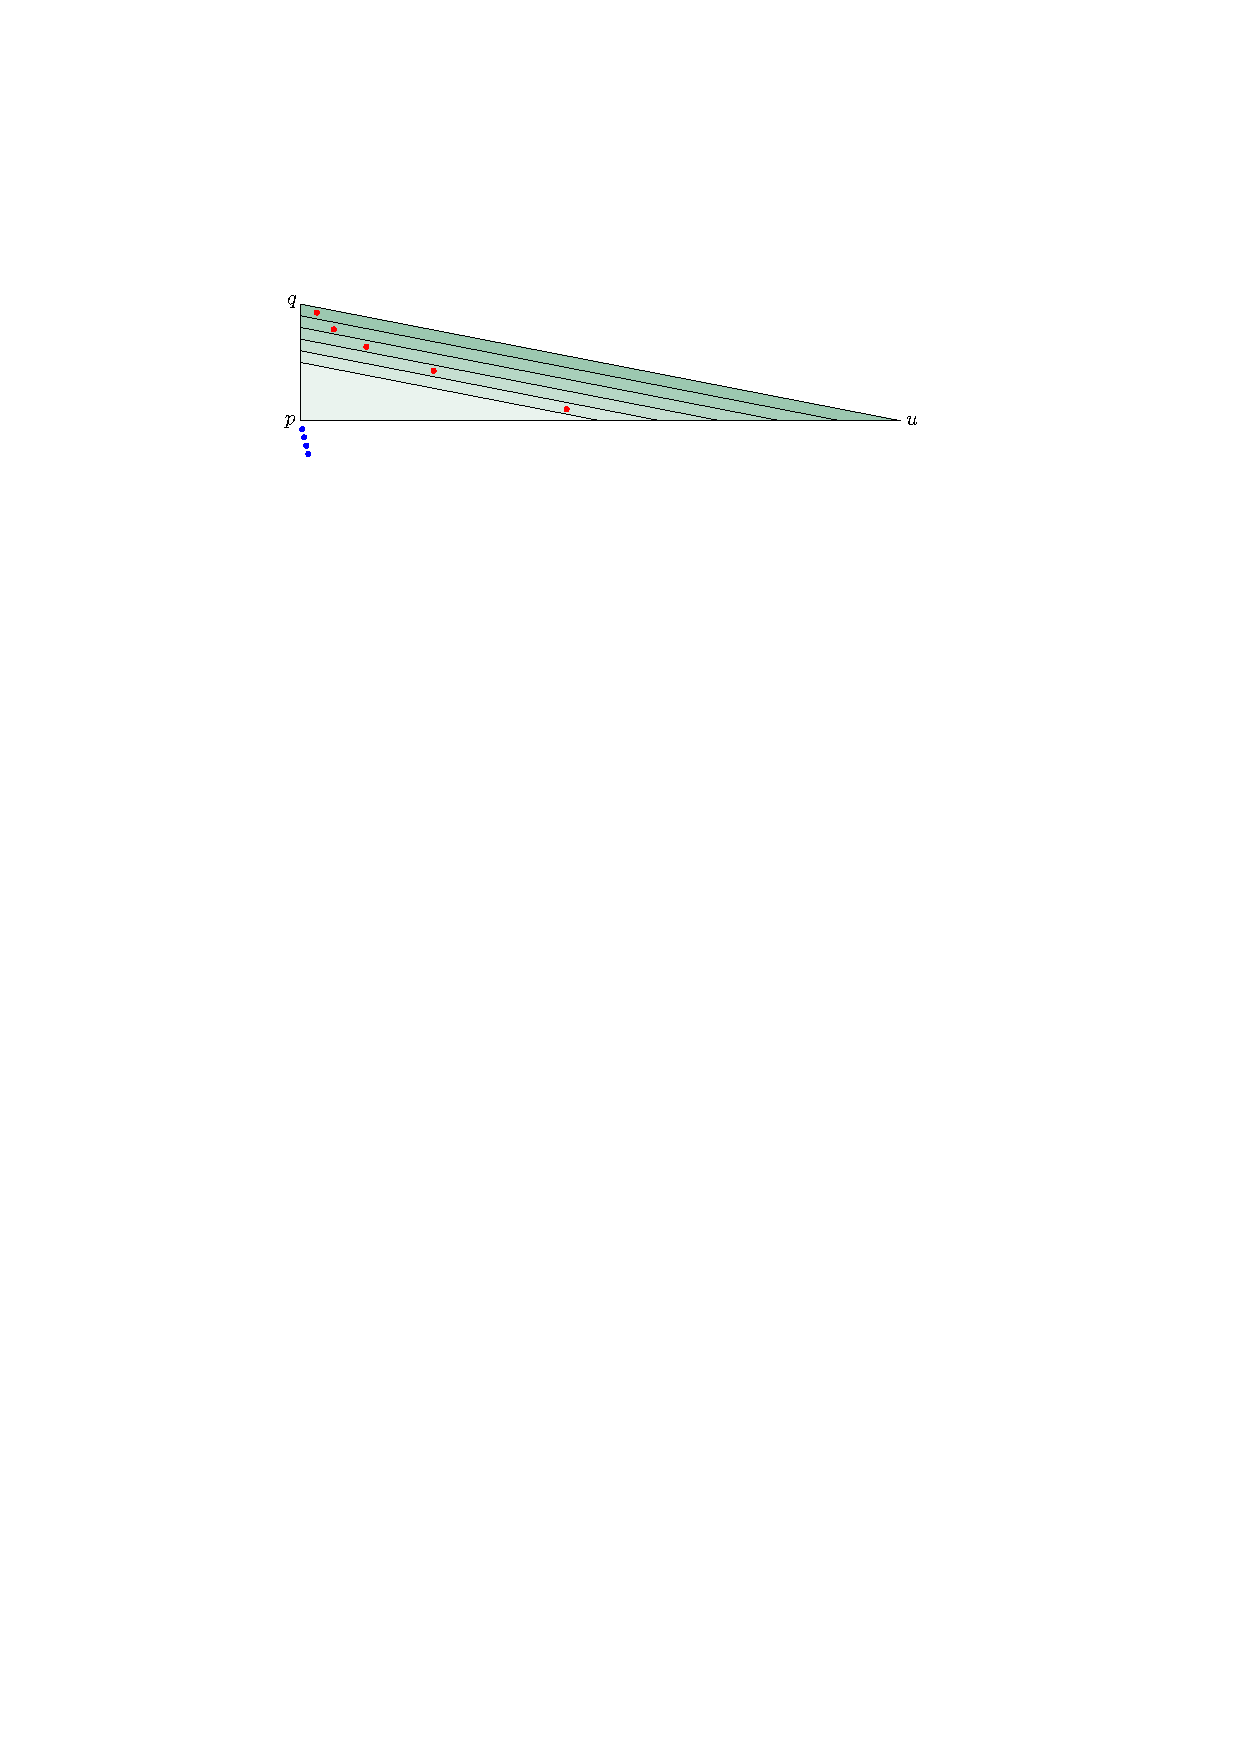
\includegraphics{../figs/triangle_lower_bound}
        \caption{An Illustration of the construction of
           \lemref{l:b:triangles}.}
        \figlab{tri_low_bd}
    \end{figure}

    For $i \in \IRX{h}$ and $j \in \IRX{n}$, let
    \begin{align*}
      \pb_i = \bigl(2^{i+1}, 1 - i/h \bigr)
      \qquad \text{ and }\qquad
      \pc_j = \bigl(\tfrac{j}{n}-1, -\tfrac{j}{n} \bigr),
    \end{align*}
    and let $\PS = \{ \pb_1, \ldots, \pb_h, \pc_1, \ldots, \pc_n\}$,
    see \figref{tri_low_bd}.  Observe that
    $\cpX{\PS} = \dY{\pc_1}{\pc_2} = \sqrt{2}/n$, and as such we have
    that
    $\spreadX{\PS} = n \cdot \diamX{\PS}/\sqrt{2} \leq n(4\Phi + 2n)
    \leq 8 \Phi n$, as $\Phi \geq n$.  Observe that
    \begin{equation*}
        \DotProd{\pb_{i+1} - \pb_i}{v}%
        =%
        \DotProd{(2^{i+1},-\tfrac{1}{h})}{ \bigl(\tfrac{1}{8\Phi h},
           1\bigr)}
        \leq
        \tfrac{4\Phi}{8\Phi h} - \tfrac{1}{h} < 0.
    \end{equation*}
    That is, the points $\pb_1, \ldots, \pb_i$ are increasing in
    distance from $\Line$.
        
    Let $\triangle_{i,j}$ be the homothet of $\triangle$, that has its
    bottom left corner at $\pc_j$, and its hypotenuse passes through
    $\pb_i$. By the above,
    $\PS(i,j) = \triangle_{i,j} \cap \PS = \{ \pc_j, \pb_i, \pb_{i+1},
    \ldots \pb_h \}$.  Any $(1+\eps)$-spanner for $\PS(i,j)$ must
    contain the edge $\pc_j \pb_i$. Indeed, we have, for any $k$, that
    $2^{k+1} \leq \dY{\pc_j}{\pb_{k}} \leq 2^{k+1} +3$. As such, any
    path on a graph induced on $\PS(i,j)$ from $\pc_j$ to $\pb_i$ that
    uses (say) a midpoint $\pb_k$, for $k >i$, must have dilation at
    least
    \begin{equation*}
        \frac{\dY{\pc_j}{\pb_k} +
           \dY{\pb_k}{\pb_i}}{\dY{\pc_j}{\pb_{i}}}
        \geq%
        \frac{2^{k+1} + 2^{k} }{2^{i+1} + 3}
        \geq%
        \frac{3 \cdot 2^{i+1} }{(1+3/4) 2^{i+1} }
        =
        \frac{12}{7}
        >
        \frac{3}{2}.
    \end{equation*}
        
    Thus, any $\triangle$-local $3/2$-spanner for homothets of
    $\triangle$, must contain the edge $\pb_i \pc_j$, for any
    $i \in \IRX{h}$ and $j \in \IRX{n}$. Thus, such a spanner must
    have $ \Omega( n \log \Phi)$ edges, as claimed.
